% ============================================================================
% Body of the MOSAIC preprint (\input from main.tex)
% ============================================================================

\section{Introduction}
A spatial transcriptomics study rarely admits a single ``correct'' analysis. Between raw
counts and a figure of spatial domains lie a dozen forks: how to normalize, how many
highly variable genes (HVGs) to keep, how many principal components, whether the
neighborhood graph is $k$-nearest-neighbor or radius-based, whether clustering uses Leiden
\citep{traag2019louvain} or Louvain \citep{blondel2008fast} and at what resolution, and
which test declares a gene spatially variable \citep{moran1950notes, svensson2018spatialde,
weber2023nnsvg}. Each fork has published precedent, so each is individually defensible. Yet
the analyst typically walks \emph{one} path and reports its endpoint as though it were the
destination.

This is the ``garden of forking paths'' \citep{gelman2013garden}: even absent any intent to
cherry-pick, the sheer number of reasonable analytic choices means a reported result can be
an artifact of the path taken rather than a property of the biology. \emph{Multiverse
analysis} \citep{steegen2016increasing} and \emph{specification-curve analysis}
\citep{simonsohn2020specification} respond by running \emph{all} defensible analyses and
reporting the distribution of outcomes---an approach dramatically validated when many teams
analyzing one neuroimaging dataset reached divergent conclusions
\citep{botvinik2020variability}.

\paragraph{Analytical versus technical reproducibility.} A growing literature audits the
\emph{technical} reproducibility of spatial platforms---how measurements vary from
instrument to instrument or protocol to protocol. MOSAIC instead audits \emph{analytical}
reproducibility: holding the data fixed, how much do conclusions vary across the pipelines a
competent analyst might reasonably choose? The two are complementary, but the analytical
degrees of freedom in spatial transcriptomics are large and, to date, largely
uncharacterized on real tissue.

\paragraph{Contributions.} (i) A parametric, bit-reproducible spatial-transcriptomics
pipeline in which every analytic choice is a configuration variable, enabling curated or
exhaustive sweeps of the multiverse (\S\ref{sec:pipeline}, \S\ref{sec:arch}). (ii) The
\emph{Spatial Stability Score} $S^3$, an interpretable family of stability metrics at the
level of spots, genes, and headline summaries, with arbitrary cluster labels aligned across
pipelines by optimal assignment (\S\ref{sec:s3}), plus a formal complexity analysis
(\S\ref{sec:complexity}). (iii) An empirical instability audit spanning mouse-brain and
human-tumor tissue with statistical tests, an anatomy-grounded validation, a variance
decomposition that identifies the single most consequential choice, a demonstration that
fragility concentrates at biological boundaries (and survives a depth-stratified control on
tumor tissue), and a demonstration that instability
propagates into downstream machine-learning performance (\S\ref{sec:results}--%
\S\ref{sec:downstream}).

\section{Related work}
\citet{steegen2016increasing} formalized the multiverse and \citet{simonsohn2020specification}
the specification curve; \citet{gelman2013garden} articulated why analytic flexibility
matters even without $p$-hacking, and \citet{botvinik2020variability} demonstrated its
consequences empirically. Standard spatial pipelines build on SCANPY
\citep{wolf2018scanpy} and Squidpy \citep{palla2022squidpy}, with community detection by
Louvain \citep{blondel2008fast} or Leiden \citep{traag2019louvain} and spatially-variable-gene
detection by Moran's $I$ \citep{moran1950notes}, SpatialDE \citep{svensson2018spatialde}, or
nnSVG \citep{weber2023nnsvg}. Benchmarks typically rank methods against a reference; we
instead quantify \emph{within-analyst} instability across defensible pipelines and turn it
into an actionable, spatially resolved metric.

\section{Methods}

\subsection{Specification space}
\label{sec:specspace}
We treat each analytic stage as an axis (Table~\ref{tab:space}). The full Cartesian product
exceeds $200$ combinations; following specification-curve practice we evaluate a
\emph{curated} set of \Nspecs{} pipelines spanning canonical, conservative, aggressive, and
extreme-but-defensible choices, so the set remains interpretable as a matrix (the full
listing is Figure~\ref{fig:specspace}).

\begin{table}[t]
  \centering
  \caption{The analytical specification space. Curated pipelines sample defensible
  combinations of these axes.}
  \label{tab:space}
  \small
  \begin{tabular}{ll}
    \toprule
    Stage & Options \\
    \midrule
    Normalization & log1p, square-root, total-count \\
    Feature selection & Seurat / Cell Ranger HVGs; $\{2000, 3000, 5000\}$ genes \\
    Dimensionality (PCA) & $\{30, 50\}$ components \\
    Neighborhood graph & $k$-nearest-neighbor, $k \in \{6, 10, 15\}$ \\
    Clustering & Leiden / Louvain; resolution $\in \{0.3, 0.5, 0.8, 1.2\}$ \\
    Spatially variable genes & Moran's $I$, FDR $< 0.05$ (Benjamini--Hochberg) \\
    \bottomrule
  \end{tabular}
\end{table}

\subsection{Parametric pipeline}
\label{sec:pipeline}
Given a specification $s$, the pipeline maps raw counts to a clustered {\tt AnnData}
\citep{virshup2023anndata} object and a table of Moran's $I$ statistics. Every stochastic
step is seeded ($\texttt{random\_state}=42$), and each pipeline re-derives its normalized
matrix from the stored raw counts so no information leaks between specifications. Leiden uses
the \texttt{leidenalg} backend; Louvain is driven through igraph's resolution-aware
multi-level optimization so the resolution axis is comparable across algorithms.
Spatially-variable-gene detection builds a spatial neighbor graph and computes Moran's $I$
with a permutation null, retaining Benjamini--Hochberg FDR-adjusted significance.

\subsection{The Spatial Stability Score}
\label{sec:s3}
Let $\mathcal{S}$ be the set of specifications, $|\mathcal{S}| = N$, and let $c_s(i) \in
\{1, \dots, K_s\}$ denote the cluster label of spot $i$ under specification $s$. Because
cluster labels are arbitrary, direct comparison of $c_s$ and $c_{s'}$ is meaningless; we
first align every specification to a fixed reference $s_0$.

\paragraph{Optimal label alignment.} Define the contingency (overlap) matrix
$M^{(s)} \in \mathbb{Z}_{\ge 0}^{K_{s_0} \times K_s}$ between the reference and specification
$s$,
\begin{equation}
  M^{(s)}_{ab} \;=\; \bigl| \{\, i : c_{s_0}(i) = a \ \wedge\ c_s(i) = b \,\} \bigr|,
\end{equation}
i.e.\ $M^{(s)}_{ab}$ counts spots that reference cluster $a$ and spec-$s$ cluster $b$ share.
An alignment is an injection $\pi_s$ from spec-$s$ labels to reference labels. We choose the
alignment of maximum total overlap,
\begin{equation}
  \pi_s \;=\; \arg\max_{\pi}\ \sum_{b=1}^{K_s} M^{(s)}_{\pi(b),\, b},
\end{equation}
which is a linear assignment problem solved by the Hungarian algorithm
\citep{kuhn1955hungarian} on the cost matrix $C^{(s)} = -M^{(s)}$ in $O(K^3)$ time, with
$K = \max(K_{s_0}, K_s)$; labels with no reference match receive fresh identifiers. Write the
aligned labels $\tilde c_s(i) = \pi_s(c_s(i))$.

\paragraph{Per-spot stability.} With labels made comparable, the per-spot stability is the
frequency of the modal (consensus) aligned label:
\begin{equation}
  S^3_{\mathrm{spot}}(i) \;=\; \frac{1}{N} \max_{\ell}\ \bigl| \{\, s \in \mathcal{S} :
  \tilde c_s(i) = \ell \,\} \bigr| \;\in\; \bigl[\tfrac{1}{N}, 1\bigr].
\end{equation}

\paragraph{Per-feature stability.} For a gene $g$, let $\mathbb{1}[g \in \mathrm{SVG}_s]$
indicate FDR-significant Moran's $I$ in specification $s$; then
\begin{equation}
  S^3_{\mathrm{gene}}(g) \;=\; \frac{1}{N} \sum_{s \in \mathcal{S}}
  \mathbb{1}[g \in \mathrm{SVG}_s].
\end{equation}

\paragraph{Headline and label-free summaries.} For a scalar metric $m$ (e.g.\ the domain
count) we report its mean, standard deviation, and range across $\mathcal{S}$. As a
label-free complement to the aligned $S^3$, we report the mean pairwise Adjusted Rand Index
\citep{hubert1985comparing} between specifications' partitions, which requires no alignment.

\subsection{Statistical analyses}
\label{sec:stats}
\paragraph{Permutation null for regional stability.} To test whether an anatomical region is
more stable than chance, we fix the per-spot scores $\{S^3(i)\}$ and the multiset of region
labels $\{r(i)\}$ and draw $B = 1000$ random permutations $\sigma$ of the region assignment,
preserving region sizes. For region $R$, the null mean is $\bar{S}^3_R(\sigma) =
\operatorname{mean}_{\{i : \sigma(r)(i) = R\}} S^3(i)$, and the one-sided empirical $p$-value is
\begin{equation}
  p_R \;=\; \frac{1 + \bigl|\{\, b : \bar{S}^3_R(\sigma_b) \ge \bar{S}^3_R \,\}\bigr|}
  {B + 1},
\end{equation}
with the add-one correction giving a conservative estimate. This asks whether region
membership explains stability beyond a random grouping of the same sizes.

\paragraph{Variance decomposition.} We regress the domain count on all analytical axes,
$\texttt{n\_domains} \sim \text{normalization} + \text{HVG method} + \text{HVG }n +
\text{resolution} + \text{algorithm} + k + \text{PCA}$, and report each axis's share of
explained variance via a Type-II ANOVA (sum-of-squares normalized to the total), including
only axes that vary.

\paragraph{Bootstrap, confound, and convergence.} We bootstrap specifications ($1000$
resamples) for $95\%$ confidence intervals on per-region $S^3$; correlate per-spot $S^3$ with
total UMI counts to test for a sequencing-depth confound; and subsample specification sets of
increasing size to confirm $S^3$ estimates converge.

\subsection{Computational complexity}
\label{sec:complexity}
Let $S$ be spots, $G$ genes, $H \le G$ retained HVGs, $d$ PCA components, $k$ graph
neighbors, $P$ Moran's-$I$ permutations, $K$ clusters, and $N$ specifications. Per
specification the dominant costs are approximate PCA via randomized SVD, $O(SHd)$; the
approximate $k$-NN graph, $O\!\left(Sk\,d \log S\right)$; community detection, $O(Sk\cdot I)$
for $I$ iterations; and permutation-based Moran's $I$ on a spatial graph with $O(S)$ edges,
$O(PSH)$. The permutation SVG step dominates in practice, giving
\begin{equation}
  T_{\text{spec}} \;=\; O\!\left(SHd + PSH\right), \qquad
  T_{\text{sweep}} \;=\; O\!\left(N\,(SHd + PSH)\right).
\end{equation}
Cross-spec alignment adds $O(N K^3)$ (Hungarian), negligible for $K \ll S$. Space is
$O(\mathrm{nnz})$ for the sparse counts, $O(SH)$ for the dense normalized matrix, $O(Sd)$ for
the embedding, and $O(SN)$ for the aligned label matrix used in $S^3$ aggregation, whose
per-spot modal reduction is $O(SN)$ time. Because the $N$ specifications are independent, the
sweep is embarrassingly parallel: with $W$ workers the wall-clock is
$O\!\left(N(SHd + PSH)/W\right)$.

\subsection{Software architecture and parallel execution}
\label{sec:arch}
MOSAIC is organized as a small, testable library (Figure~\ref{fig:arch}). A data loader
returns an {\tt AnnData} object and stashes raw counts in a dedicated layer; a
configuration file enumerates the specification space; a parametric \texttt{SpatialPipeline}
consumes one specification and emits a clustered object plus a Moran's-$I$ table; a
\texttt{StabilityScorer} aggregates results into the $S^3$ family; and a visualization layer
renders figures. Sweeps use content-hashed, idempotent checkpoints, so re-running only
computes new specifications---enabling incremental growth of the multiverse and safe
recovery from interruption.

Because specifications share no state, execution scales trivially across cores or a compute
cluster: each $(s)$ is a pure function of the shared prepared data and its own seed, so the
sweep maps cleanly onto process pools, batch schedulers (e.g.\ Slurm array jobs), or ephemeral
remote workers, with results reduced by the scorer. An exhaustive multiverse of thousands of
specifications is therefore reachable by horizontal scaling without changing the pipeline.

\begin{figure}[t]
  \centering
  \begin{tikzpicture}[
      font=\small,
      node distance=6mm and 9mm,
      box/.style={draw=darkblue!70, rounded corners, fill=panelgray, align=center,
        inner sep=4pt, minimum height=8mm, text width=20mm},
      data/.style={draw=accent!70, rounded corners, fill=accent!8, align=center,
        inner sep=4pt, minimum height=8mm, text width=20mm},
      arr/.style={-{Stealth[length=2mm]}, darkblue!80, thick}]
    \node[data] (raw) {Raw counts\\{\tt AnnData}};
    \node[box, right=of raw] (norm) {Normalize};
    \node[box, right=of norm] (hvg) {HVG\\selection};
    \node[box, right=of hvg] (pca) {PCA};
    \node[box, below=8mm of pca] (graph) {$k$-NN\\graph};
    \node[box, left=of graph] (clust) {Leiden /\\Louvain};
    \node[box, left=of clust] (svg) {Moran's $I$\\(SVG)};
    \node[data, left=of svg] (out) {Per-spec\\outputs};
    \node[data, below=8mm of out] (scorer) {Stability\\Scorer};
    \node[box, right=of scorer] (s3) {$S^3$, ARI,\\stats};
    \node[box, right=of s3] (fig) {Figures /\\paper};
    \node[draw=darkblue!40, dashed, above=1mm of norm, xshift=10mm, text width=42mm,
      align=center, font=\footnotesize\itshape] (cfg) {config: one of $N$ specifications};

    \draw[arr] (raw) -- (norm); \draw[arr] (norm) -- (hvg); \draw[arr] (hvg) -- (pca);
    \draw[arr] (pca) -- (graph); \draw[arr] (graph) -- (clust); \draw[arr] (clust) -- (svg);
    \draw[arr] (svg) -- (out); \draw[arr] (out) -- (scorer);
    \draw[arr] (scorer) -- (s3); \draw[arr] (s3) -- (fig);
    \draw[arr, dashed, darkblue!50] (cfg) -- (norm);
    \draw[arr, dashed, darkblue!50] (cfg.east) to[bend left=12] (clust.north);
  \end{tikzpicture}
  \caption{MOSAIC dataflow. A single shared prepared object feeds $N$ independent,
  configuration-driven pipeline runs (top row and back); each emits per-spec outputs that the
  stability scorer reduces into the $S^3$ family and figures. Independence of specifications
  makes the sweep embarrassingly parallel.}
  \label{fig:arch}
\end{figure}

\section{Experiments}
We evaluate on two independent 10x Genomics Visium mouse-brain coronal sections distributed
with Squidpy \citep{palla2022squidpy}: a primary H\&E section ($\Nspots{}$ spots,
$\Ngenes{}$ genes) and, for generalization, an independently prepared fluorescence section
($2{,}800$ spots). Both ship real histology and a curated anatomical annotation (15 regions:
cortical layers, hippocampus, thalamus, striatum, fiber tracts, ventricle, and more) used as
ground truth. All \Nspecs{} specifications are seeded; determinism is verified by re-running a
fixed specification and confirming identical spot-level labels. Runtime is roughly one minute
per specification on a single Apple-silicon CPU. To test whether fragility is worse where the
biological stakes are higher, we additionally run the full multiverse on a public 10x Visium
human breast-cancer section (invasive ductal carcinoma; 3{,}798 spots), applying only minimal
shared gene quality control (dropping genes detected in fewer than ten spots) so that every
specification sees the same gene universe.

\section{Results}
\label{sec:results}
\paragraph{Headline instability.} The number of recovered spatial domains ranges from
\ClustMin{} to \ClustMax{} across the multiverse (mean $\ClustMean{} \pm \ClustStd{}$;
Figure~\ref{fig:montage}, \ref{fig:speccurve}). Label-invariant agreement is modest: the mean
pairwise Adjusted Rand Index between specifications' partitions is \AriMean{} (range
$\AriMin{}$--$\AriMax{}$), so different pipelines carve the tissue into materially different
domains rather than merely relabeling one partition.

\paragraph{Where the tissue is (un)stable.} Per-spot $S^3$ (Figure~\ref{fig:map}) concentrates
instability at region boundaries and ventricular/low-signal areas while region interiors are
stable: \SpotStableFrac{} of spots are robust ($S^3 \ge 0.8$) and \SpotFragileFrac{} fragile
($S^3 < 0.5$). Magnified real-tissue insets confirm that fragile zones coincide with
morphological transitions (Figure~\ref{fig:insets}), and canonical marker genes recover the
expected neuroanatomy (Figure~\ref{fig:markers}). Stratifying spots into domain
\emph{boundaries} and \emph{interiors} makes this quantitative: mean $S^3$ at boundaries is
\BoundaryS{} versus \InteriorS{} in interiors, a gap of \StakesGap{} that a label-shuffle
permutation null rejects as chance ($p\,\StakesP{}$; Figure~\ref{fig:stakes}). Analytical
fragility concentrates precisely at the biological transitions where a domain assignment is
most consequential.

\paragraph{Stability tracks biology, not analysis.} Consensus domains recover known anatomy,
with each specification agreeing with the reference annotation at mean ARI \RefAriMean{} (up
to \RefAriMax{}; Figure~\ref{fig:refval}). Per-region $S^3$ is highest in transcriptomically
distinct structures (thalamus, hippocampus, cortical layers) and lowest at the lateral
ventricle and mixed cortical zones. A label-permutation null confirms \RegionsStable{} of
\NregionsTotal{} regions are stable beyond chance ($p < 0.05$;
Figure~\ref{fig:permutation}), and a confound check shows $S^3$ is essentially uncorrelated
with sequencing depth (Pearson $r = \ConfoundR{}$; Figure~\ref{fig:confound}), so instability
is biological rather than a low-quality-spot artifact.

\paragraph{One choice dominates.} A Type-II variance decomposition attributes \VarTopFrac{} of
the domain-count variance to a single choice---clustering \VarTopAxis{}---with all other axes
each contributing at most a few percent (Figure~\ref{fig:variance}). Standardizing resolution
is thus far more consequential than any other step.

\paragraph{Which genes are robust.} Per-gene $S^3$ separates genes called spatially variable
regardless of pipeline (\GeneRobustFrac{} with $S^3 > 0.8$) from those whose SVG status flips
with the analysis (\GeneFragileFrac{} with $S^3 < 0.5$; Figure~\ref{fig:genes}). Restricting
to genes tested in every specification, individual SVG calls still churn substantially.
Concretely (Figure~\ref{fig:fragility}), the most contested gene sits on the FDR knife-edge:
it is declared a significant spatially variable gene in most---but not all---defensible
pipelines, so a study reporting it (or its absence) from a single pipeline would be equally
``correct'' either way. A per-gene $S^3$ flags exactly this contingency, which is the concrete
form of fragility-aware reporting we advocate.

\paragraph{Generalization.} The pattern is not specific to one sample. The full sweep on the
independent fluorescence section yields a per-spot $S^3$ distribution with a comparable robust
core and fragile tail and a similar mean pairwise ARI (Figure~\ref{fig:cross}); the $S^3$
distributions of the two sections are essentially conserved.

\paragraph{Higher-stakes human tumor tissue.} Running the multiverse on a human breast-cancer
section reproduces the core findings on clinically consequential tissue. Boundary fragility
persists and is modestly larger than in brain: mean $S^3$ is \TumorBoundaryS{} at
consensus-domain boundaries versus \TumorInteriorS{} in interiors (gap \TumorGap{}, permutation
$p\,\TumorStakesP{}$), compared with a \StakesGap{} gap in brain. Tumor tissue does, however,
introduce a genuine technical confound absent in brain: per-spot $S^3$ correlates with
sequencing depth ($r=\TumorConfoundR{}$, versus $\ConfoundR{}$ in brain), and boundary spots are
systematically shallower. We therefore test the gap with a depth-stratified block-permutation
null---binning spots by depth decile and shuffling the boundary/interior label only within each
bin, so the null preserves each group's depth distribution. The gap survives
($p\,\TumorDepthP{}$), so it is not merely an artifact of low-coverage spots. Finally, the
dominant analytical axis does \emph{not} change with tissue type: clustering resolution still
explains the most domain-count variance (\TumorVarTopFrac{}, versus \VarTopFrac{} in brain),
an honest null for the hypothesis that the most consequential choice is tissue-dependent. Thus
the fragility phenomenon, its concentration at boundaries, and its leading cause all transfer
to human tumor tissue, while the tumor setting sharpens the importance of controlling for
sequencing depth (Figure~\ref{fig:tumorstakes}).

\begin{figure}[t]
  \centering
  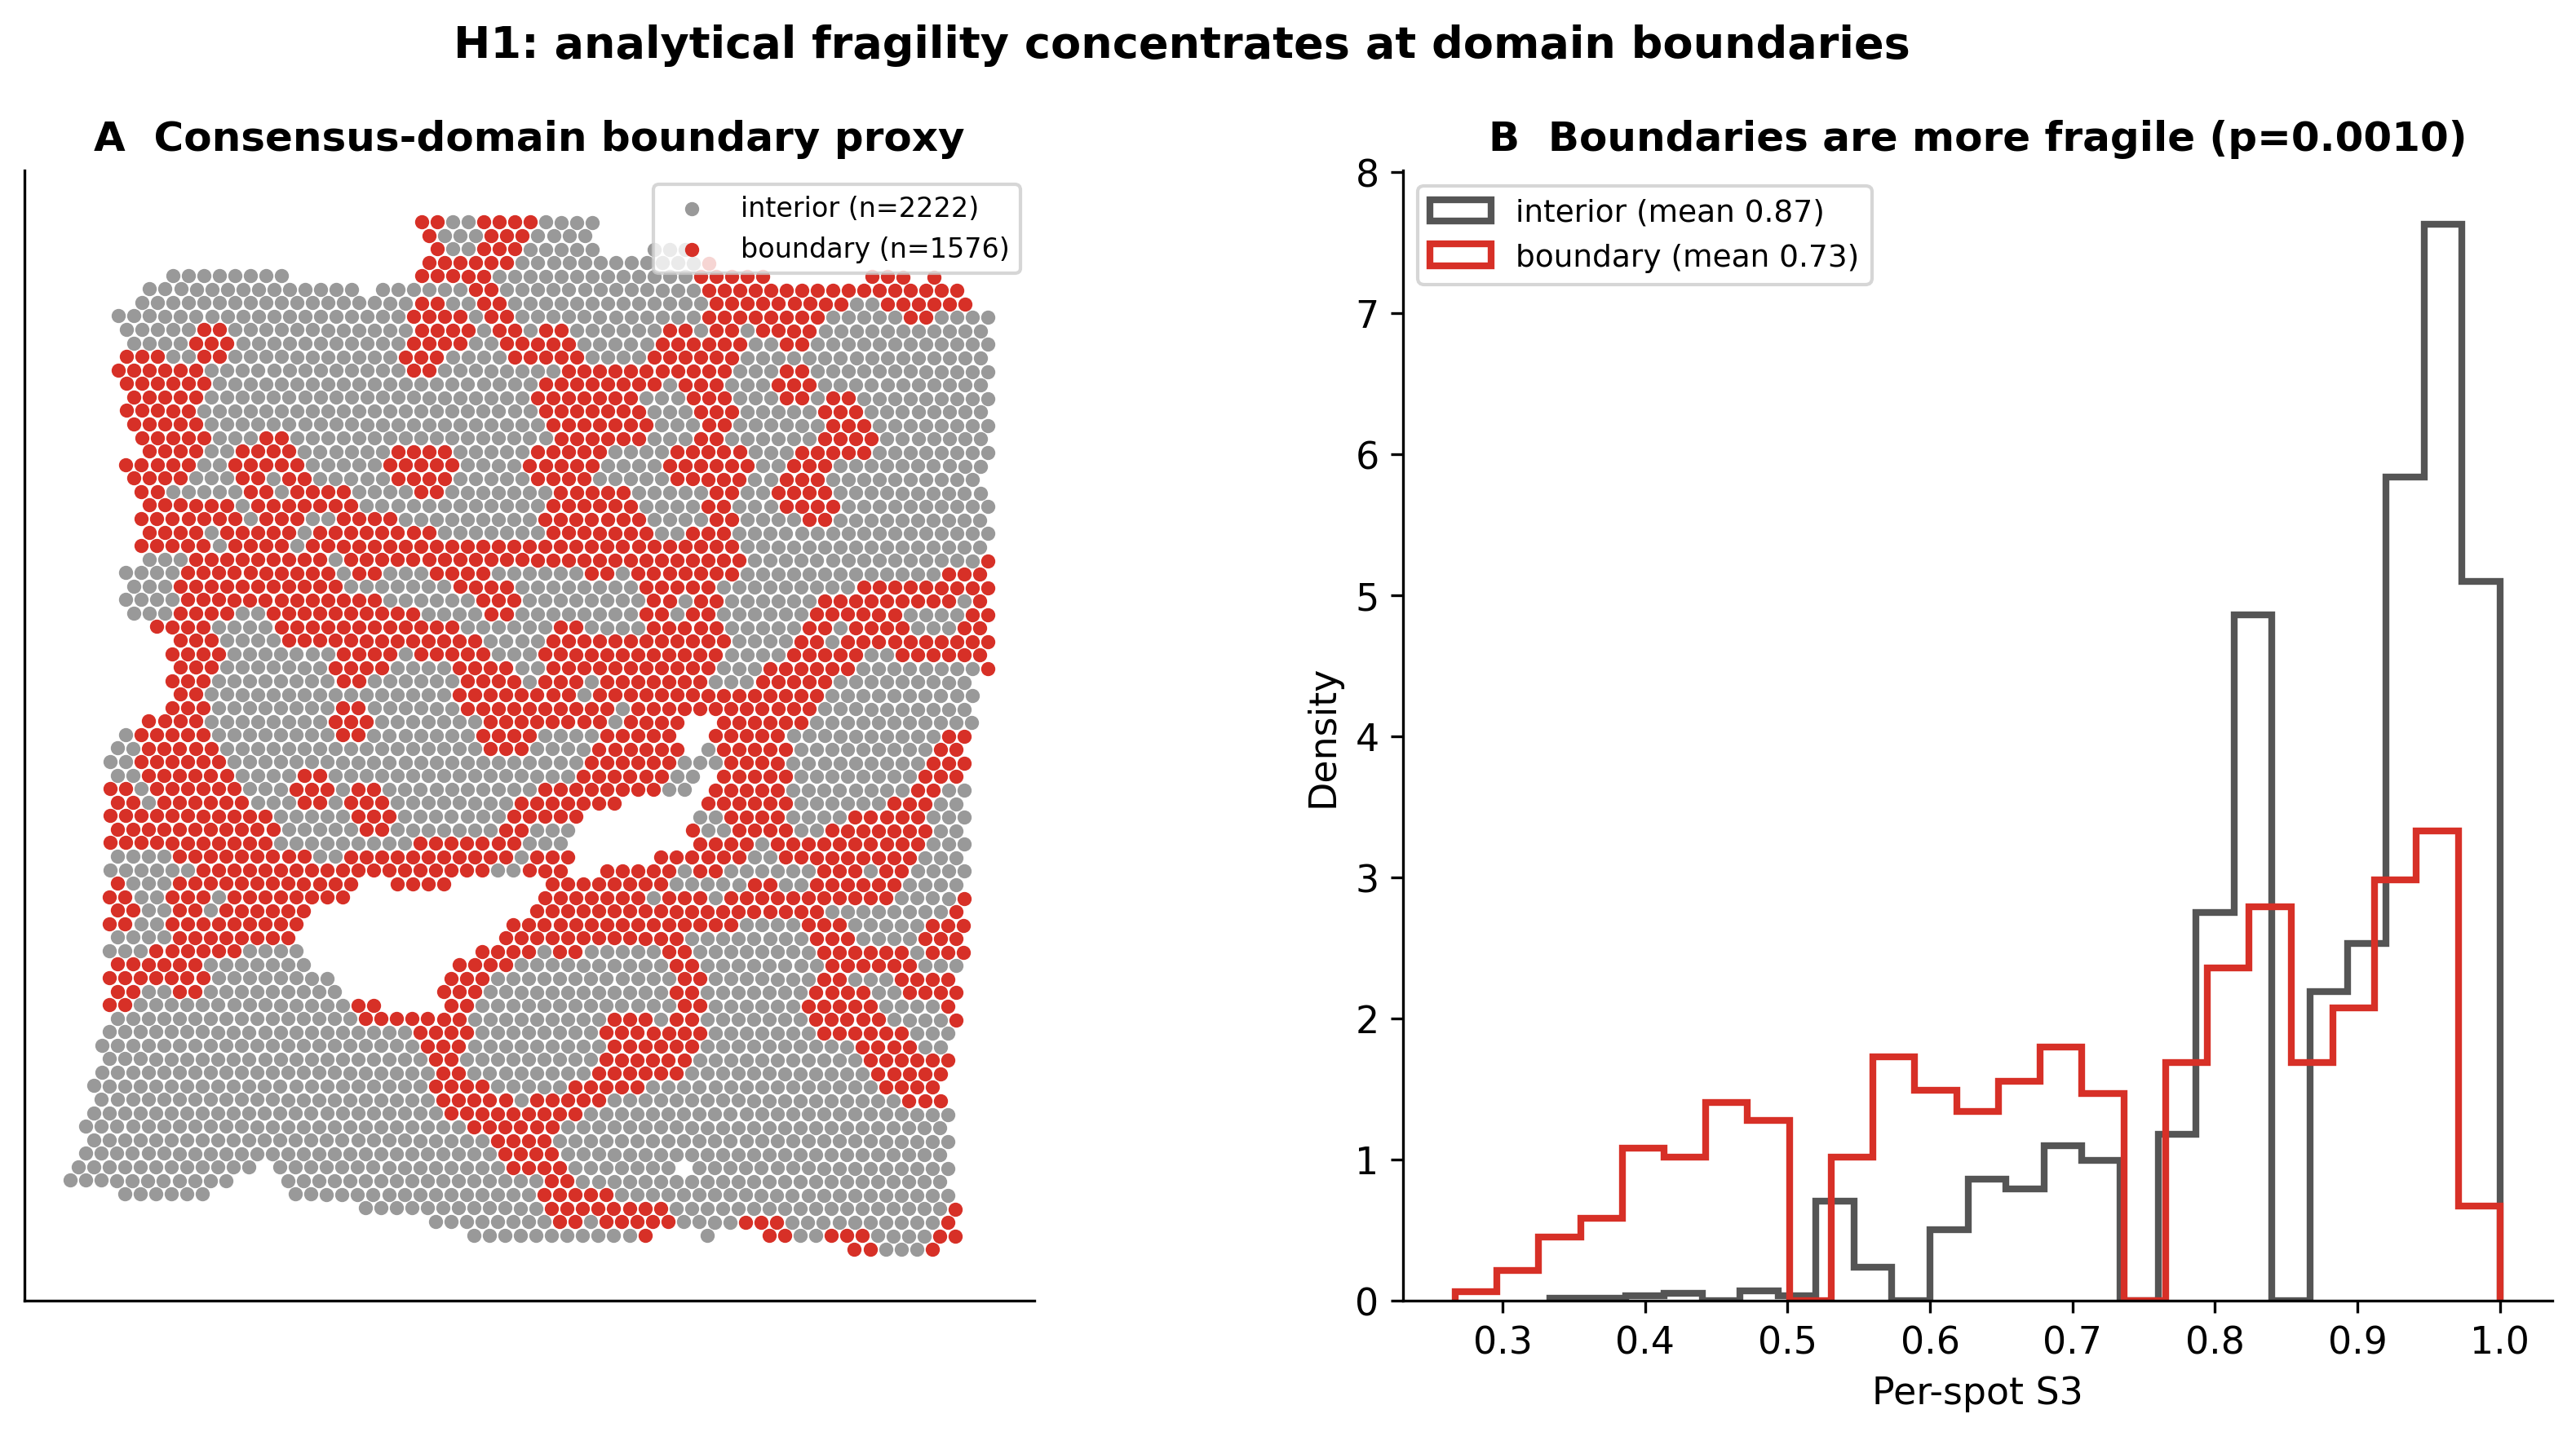
\includegraphics[width=\linewidth]{../results/breast_cancer/figures/13_stakes_stratified.png}
  \caption{Fragility at domain boundaries on human breast-cancer tissue. Boundary spots (red)
  are significantly more fragile than interiors, replicating the mouse-brain result on a
  higher-stakes tumor section; the gap survives a depth-stratified permutation null.}
  \label{fig:tumorstakes}
\end{figure}

\section{Downstream machine-learning implications}
\label{sec:downstream}
Instability is not merely descriptive: the representation a model consumes is itself
pipeline-dependent. To quantify the consequence, we trained a cross-validated logistic-regression
classifier to predict anatomical region from each specification's PCA embedding
(Figure~\ref{fig:downstream}). Accuracy ranges from \DownstreamAccMin{} to \DownstreamAccMax{}
across the multiverse---a \DownstreamRangePP{}~percentage-point swing attributable solely to
upstream analytical choices, with no change to the model or its hyperparameters. The effect is sharper for
\emph{calibration} than for accuracy: the multiclass Brier score of the same classifier ranges
from \BrierMin{} to \BrierMax{} across pipelines---nearly a two-fold swing in how well the
model's predicted probabilities are calibrated---driven entirely by upstream analytical
choices. A researcher who fixes a single pipeline therefore inherits an unquantified,
pipeline-dependent bias in downstream performance and calibration; reporting the $S^3$ of the
features and domains a model is trained on makes that dependence explicit.

\begin{figure}[t]
  \centering
  \includegraphics[width=\linewidth]{12_downstream_ml.png}
  \caption{Downstream impact. (A) Cross-validated region-classification accuracy across the
  \Nspecs{} pipelines, sorted; the shaded band is the achievable range. (B) Accuracy versus
  the upstream clustering resolution. Pipeline choice alone moves downstream accuracy by
  \DownstreamRangePP{}~pp.}
  \label{fig:downstream}
\end{figure}

\section{Practical recommendations}
For researchers who cannot run a full multiverse, the variance decomposition
(Figure~\ref{fig:variance}) gives a concrete priority order. First, \emph{fix and report the
clustering resolution}: it accounts for \VarTopFrac{} of the variability in the recovered
domain count, dwarfing every other choice. Second, report the neighborhood-graph size $k$,
the next largest contributor. Normalization, feature-selection method, HVG count, PCA
dimensionality, and the Leiden-versus-Louvain choice each move the result only marginally and
may be set to community defaults. Finally, treat SVG calls near the significance threshold as
provisional and report a per-gene $S^3$ alongside any SVG list; likewise report the $S^3$ of
domains used as features in any downstream model.

\section{Discussion and limitations}
MOSAIC quantifies, rather than resolves, analytic ambiguity: it tells a researcher which
conclusions are robust and which are contingent, and provides a spatially resolved map of
where to place trust. The agreement between per-spot $S^3$ and reference anatomy, together with
the near-zero depth correlation, indicates $S^3$ measures biological rather than merely
analytical uncertainty. Limitations include the use of a curated (not exhaustive) set of
specifications; three Visium sections spanning two mouse-brain samples and one human tumor (a
broader survey across further tissues, patients, and sub-cellular-resolution platforms such as
Xenium remains important future work); and reliance on a consensus-domain boundary proxy where
pathologist annotations are unavailable. On the tumor section the $S^3$--depth correlation is
substantial, and although a depth-stratified null shows the boundary gap survives, we do not
claim a full multivariate deconfounding. The framework accommodates additional axes, datasets,
tests (it already supports Moran's~$I$ and Geary's~$C$), and stratifications without
modification.

\paragraph{Toward agentic multiverse navigation.} The curated \Nspecs{}-specification set is a
static sample of a much larger space. Because each specification returns a well-defined
stability signal, the multiverse is naturally framed as a search problem: an agent could use
Bayesian optimization or active learning to propose specifications that maximally reduce
uncertainty about $S^3$, or to map the boundary between robust and contingent regions of the
configuration space far more efficiently than uniform curation. The embarrassingly parallel
architecture (\S\ref{sec:arch}) makes such agent-driven exploration, and eventually an
exhaustive multiverse, computationally tractable.

\section{Reproducibility}
Every specification is seeded and re-derives its inputs from raw counts; sweeps are idempotent
and content-hashed. We release the code, the specification configuration, the aggregate
stability tables, the statistical outputs, and the figure scripts; the primary study
reproduces with \texttt{make repro}, and the second dataset with a single
\texttt{--dataset} flag. Analyses build on NumPy \citep{harris2020array}, SciPy
\citep{virtanen2020scipy}, scikit-learn \citep{pedregosa2011scikit}, SCANPY
\citep{wolf2018scanpy}, and Squidpy \citep{palla2022squidpy}. Data download automatically from
public Squidpy mirrors.

% ---------------------------------------------------------------------------
% Figures (placed after the text; LaTeX floats them to nearby pages)
% ---------------------------------------------------------------------------
\begin{figure}[t]
  \centering
  \includegraphics[width=\linewidth]{fig1_spec_montage.png}
  \caption{The same mouse-brain section analyzed with five defensible specifications (A--E)
  yields 8--18 spatial domains with visibly different extents; (F) the per-spot $S^3$ overlay
  summarizes agreement across the full multiverse (green robust, red fragile).}
  \label{fig:montage}
\end{figure}

\begin{figure}[t]
  \centering
  \includegraphics[width=\linewidth]{fig2_spec_curve_matrix.png}
  \caption{Specification-curve matrix. Top: number of domains, sorted across pipelines.
  Middle: each pipeline's agreement with the multiverse consensus. Bottom: for genes tested in
  every specification, whether each is a significant SVG (black) per pipeline.}
  \label{fig:speccurve}
\end{figure}

\begin{figure}[t]
  \centering
  \includegraphics[width=\linewidth]{fig3_stability_summary.png}
  \caption{(A) Per-spot $S^3$ map. (B) $S^3$ distribution over all $\Nspots{}$ spots with
  robust ($\ge 0.8$) and fragile ($<0.5$) thresholds. (C) Mean $S^3$ by data-driven consensus
  domain.}
  \label{fig:map}
\end{figure}

\begin{figure}[t]
  \centering
  \includegraphics[width=\linewidth]{05_zoomed_insets.png}
  \caption{Real H\&E tissue at a robust core versus a fragile boundary, with per-spot $S^3$
  overlays; fragile zones coincide with morphological transitions.}
  \label{fig:insets}
\end{figure}

\begin{figure}[t]
  \centering
  \includegraphics[width=\linewidth]{06_marker_genes.png}
  \caption{Spatial expression of canonical mouse-brain markers on the H\&E image; recovered
  patterns match known neuroanatomy (myelin markers in fiber tracts, \emph{Hpca} in
  hippocampus, \emph{Pcp4} in thalamus).}
  \label{fig:markers}
\end{figure}

\begin{figure}[t]
  \centering
  \includegraphics[width=\linewidth]{ed7_reference_validation.png}
  \caption{Validation against reference anatomy. (A) Row-normalized agreement between
  anatomical regions and consensus domains. (B) Mean per-spot $S^3$ per region.}
  \label{fig:refval}
\end{figure}

\begin{figure}[t]
  \centering
  \includegraphics[width=\linewidth]{13_stakes_stratified.png}
  \caption{Fragility concentrates where stakes are highest. (A) Spots split into
  consensus-domain boundaries (red) and interiors (grey). (B) Boundary spots are
  significantly more fragile (lower $S^3$) than interiors (permutation null). Where
  pathologist annotations are unavailable this uses a data-driven boundary proxy.}
  \label{fig:stakes}
\end{figure}

\begin{figure}[t]
  \centering
  \includegraphics[width=0.78\linewidth]{09_permutation_test.png}
  \caption{Per-region observed mean $S^3$ against a label-permutation null; green regions are
  stable beyond chance ($p < 0.05$).}
  \label{fig:permutation}
\end{figure}

\begin{figure}[t]
  \centering
  \includegraphics[width=0.7\linewidth]{11_confound_umi.png}
  \caption{Per-spot $S^3$ versus total UMI counts. The near-zero correlation shows $S^3$ is not
  a proxy for sequencing depth.}
  \label{fig:confound}
\end{figure}

\begin{figure}[t]
  \centering
  \includegraphics[width=0.72\linewidth]{08_variance_decomposition.png}
  \caption{Variance in domain count attributed to each analytical axis (Type-II ANOVA);
  clustering resolution dominates.}
  \label{fig:variance}
\end{figure}

\begin{figure}[t]
  \centering
  \includegraphics[width=\linewidth]{ed5_svg_stability.png}
  \caption{(A) Least stable SVG calls ranked by call frequency among commonly-tested genes.
  (B) Gene $\times$ specification concordance (black = called).}
  \label{fig:genes}
\end{figure}

\begin{figure}[t]
  \centering
  \includegraphics[width=0.85\linewidth]{14_fragility_report.png}
  \caption{Fragility-aware reporting. The most contested gene's FDR-adjusted Moran's I
  p-value across all pipelines; many defensible pipelines sit at the $p=0.05$ threshold, so
  its ``significant SVG'' status flips with the analysis. A per-gene $S^3$ makes this explicit.}
  \label{fig:fragility}
\end{figure}

\begin{figure}[t]
  \centering
  \includegraphics[width=\linewidth]{ed8_cross_dataset.png}
  \caption{Generalization across two independent mouse-brain sections (H\&E and fluorescence):
  per-spot $S^3$ maps (top) and conserved $S^3$ distributions (bottom).}
  \label{fig:cross}
\end{figure}

\begin{figure}[t]
  \centering
  \includegraphics[width=\linewidth]{ed4_spec_space.png}
  \caption{The curated specification space: each row is one pipeline with its analytical
  choices and resulting domain count.}
  \label{fig:specspace}
\end{figure}
